% 建议使用 XeLaTeX 或 LuaLaTeX 编译(更佳的中文支持)
\documentclass[UTF8,zihao=-4]{ctexart}

% 统一导言(geometry, amsmath, amssymb, amsthm, bm, hyperref, graphicx, caption, listings, xcolor, float, placeins)
\usepackage[a4paper,margin=2.5cm]{geometry}
\usepackage{amsmath,amssymb,amsthm}
\usepackage{bm}
\usepackage{hyperref}
\usepackage{graphicx}
\usepackage{caption}
\usepackage{listings}
\usepackage{xcolor}
\usepackage{float}
\usepackage{placeins}

% 图片路径
\graphicspath{{figures/}}

% 统一代码风格
\lstdefinestyle{code}{%
  language=Python,
  basicstyle=\ttfamily\small,
  numbers=left,
  numberstyle=\tiny, 
  keywordstyle=\color{blue}\bfseries,
  commentstyle=\color{teal!70!black},
  stringstyle=\color{orange!70!black},
  breaklines=true,
  frame=single,
  rulecolor=\color{black!30},
  tabsize=2,
  showstringspaces=false
}
\lstset{style=code}

\title{朴素贝叶斯:理论与实践}
\author{}
\date{\today}

\begin{document}
\maketitle

% 结构:Introduction / Theory and Formulas / Applications and Tips / Python Practice / Result / Summary

\section{引言}
朴素贝叶斯(Na\"\i ve Bayes,NB)是在\textbf{条件独立}假设下建立的概率分类器族:
\begin{equation}
 p(y\mid \mathbf{x}) \propto p(y)\,\prod_{j=1}^{d} p(x_j \mid y),
\end{equation}
其中 $y$ 为类别,$\mathbf{x}=(x_1,\dots,x_d)$ 为特征。尽管独立性假设较强,NB 在高维稀疏特征(如文本)等任务中常表现稳健,且训练、预测效率较高。

\section{原理与公式}
以高斯朴素贝叶斯(Gaussian NB)为例,对于连续特征,假设对每个类别 $c\in\{1,\dots,C\}$ 与每个特征 $j$ 有:
\begin{equation}
 x_j \mid y=c \;\sim\; \mathcal{N}(\mu_{c,j},\, \sigma^2_{c,j}).
\end{equation}
则条件似然分解为 $p(\mathbf{x}\mid y=c)=\prod_{j} \mathcal{N}(x_j\,;\,\mu_{c,j},\sigma^2_{c,j})$。结合先验 $p(y=c)$,(未归一化的) 对数后验为:
\begin{align}
 \log p(y=c\mid \mathbf{x}) 
 &\propto \log p(y=c) + \sum_{j=1}^d \log \mathcal{N}(x_j\,;\,\mu_{c,j},\sigma^2_{c,j})\\
 &\propto \log p(y=c) - \sum_{j=1}^d \Big[ \tfrac{1}{2}\log (2\pi\sigma^2_{c,j}) + \tfrac{(x_j-\mu_{c,j})^2}{2\sigma^2_{c,j}} \Big].
\end{align}
预测类别为 $\hat y = \arg\max_c \log p(y=c\mid \mathbf{x})$。参数估计可由各类别内样本的均值与方差直接得到。

\paragraph{备注} 变体包括:连续特征的 Gaussian NB;计数/二值特征的 Multinomial/Bernoulli NB(常配合拉普拉斯平滑)。若需使用概率值做后续决策,建议做概率校准。

\section{应用场景与要点}
\begin{itemize}
  \item \textbf{适用场景:} 高维稀疏文本(BOW/TF-IDF)、简单传感器数据、作为强基线。
  \item \textbf{预处理:} Gaussian NB 建议对连续特征做标准化;文本常用计数或 TF-IDF(Multinomial NB)。
  \item \textbf{类别先验:} 可用经验频率或领域知识设定。
  \item \textbf{独立性假设:} 特征强相关时性能可能下降;建议与逻辑回归/线性 SVM 等对比。
  \item \textbf{评估:} 采用交叉验证对比不同模型与超参数。
\end{itemize}

\section{Python 实战}
在章节目录内运行下述脚本,图片将保存到本目录下的 \texttt{figures/}:
\begin{lstlisting}[style=code,caption={生成朴素贝叶斯配图},label={lst:genfigs_cn}]
# 在 4_Naive Bayes 目录中执行:
python gen_naive_bayes_figures.py
\end{lstlisting}

% 将完整 Python 源码纳入文章
\lstinputlisting[style=code,caption={gen\_naive\_bayes\_figures.py 源码},label={lst:source_nb_cn}]{gen_naive_bayes_figures.py}

\section{结果}
\begin{figure}[H]
  \centering
  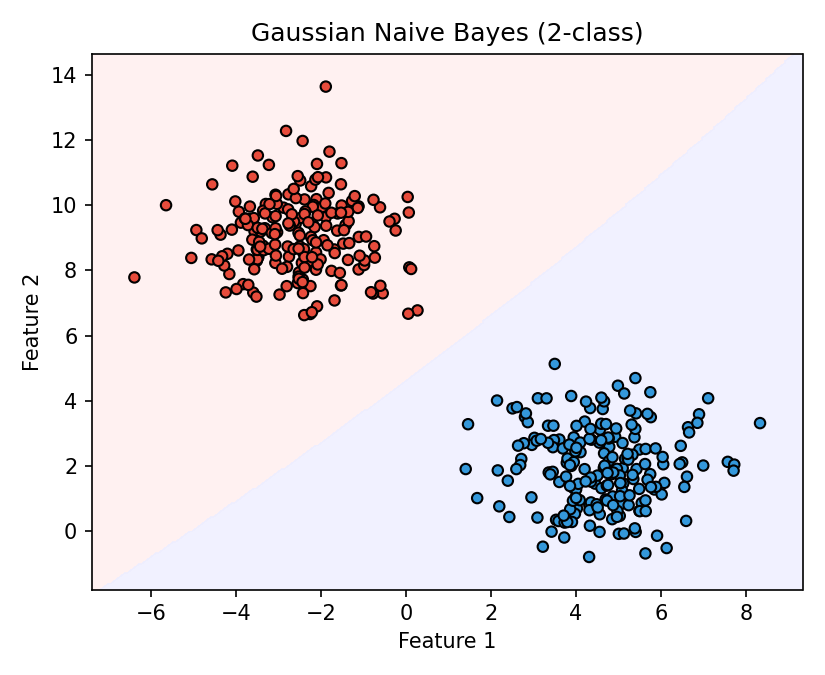
\includegraphics[width=0.9\linewidth]{gnb_decision_boundary_2class.png}
  \caption{Gaussian NB 分类边界(两类)。}
  \label{fig:gnb2_cn}
\end{figure}
\FloatBarrier

\begin{figure}[H]
  \centering
  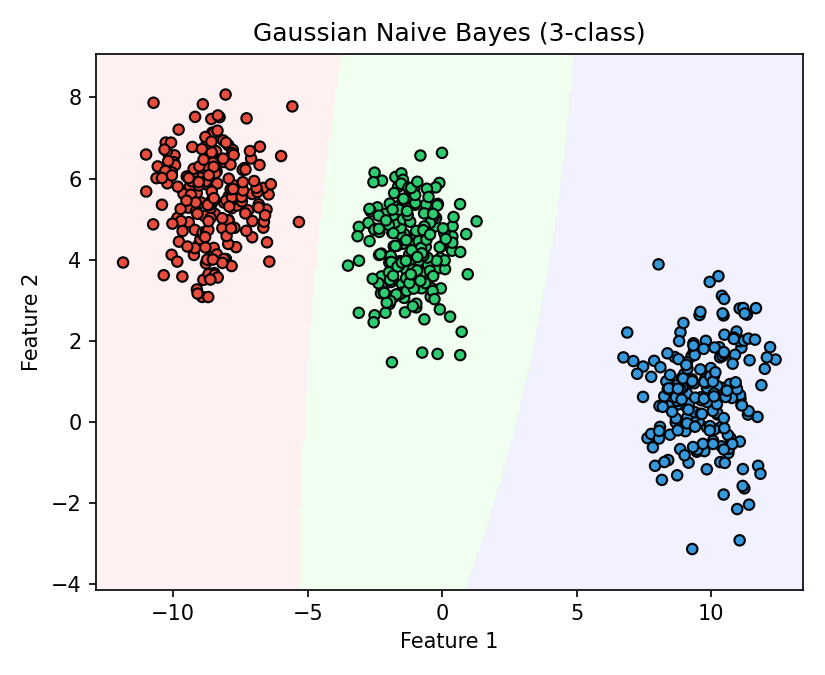
\includegraphics[width=0.9\linewidth]{gnb_decision_boundary_3class.png}
  \caption{Gaussian NB 决策区域(三类)。}
  \label{fig:gnb3_cn}
\end{figure}
\FloatBarrier

\begin{figure}[H]
  \centering
  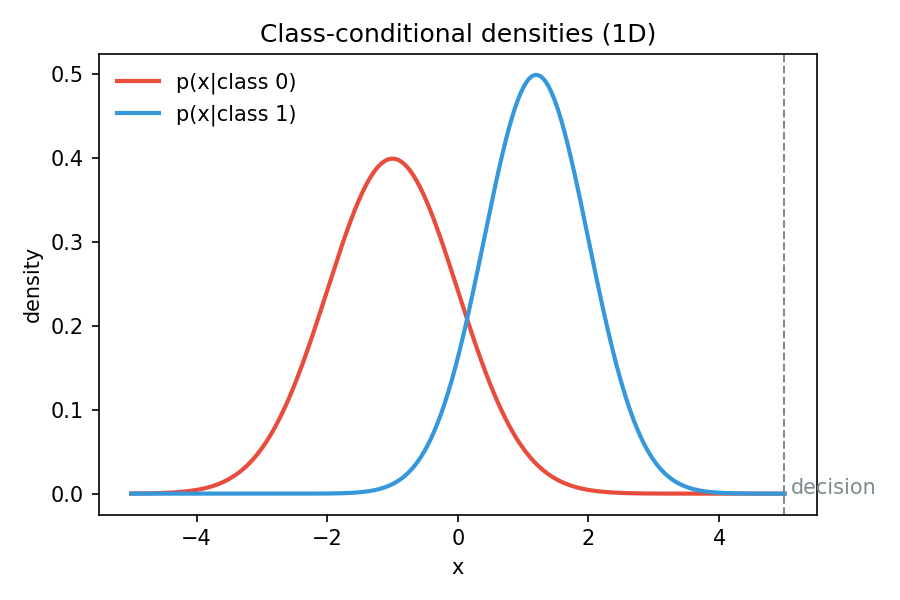
\includegraphics[width=0.9\linewidth]{class_conditional_densities_1d.png}
  \caption{一维类别条件密度与决策阈值。}
  \label{fig:dens1d_cn}
\end{figure}
\FloatBarrier

\begin{figure}[H]
  \centering
  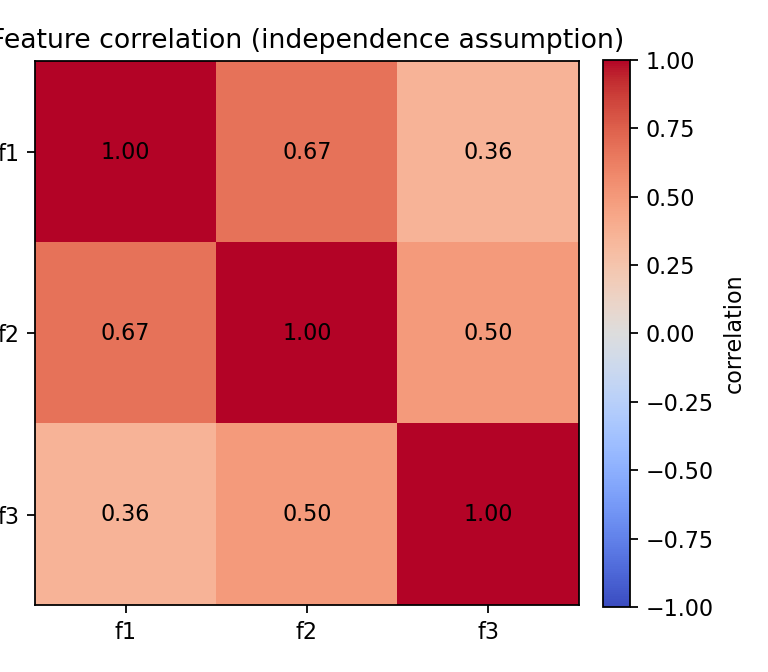
\includegraphics[width=0.9\linewidth]{feature_independence_heatmap.png}
  \caption{特征相关性热力图(独立性假设示意)。}
  \label{fig:heatmap_cn}
\end{figure}
\FloatBarrier

\begin{figure}[H]
  \centering
  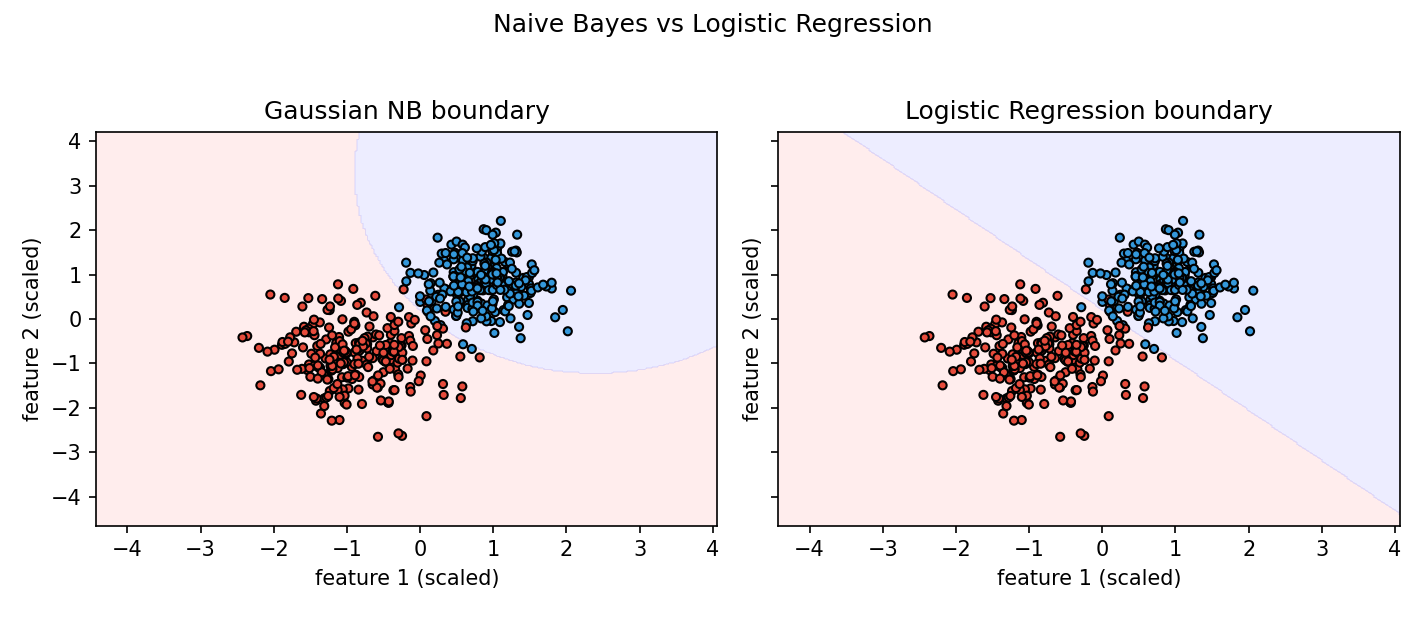
\includegraphics[width=0.95\linewidth]{gnb_vs_logreg_boundary.png}
  \caption{Gaussian NB 与逻辑回归的决策边界对比。}
  \label{fig:nb_vs_lr_cn}
\end{figure}
\FloatBarrier

\section{总结}
朴素贝叶斯以简洁可解释、训练与预测高效为特点:核心是先验与逐特征似然的乘积(条件独立)。虽然假设并非总成立,它依然是可靠的基线模型,常用于与更强的判别式模型进行对比。

\end{document}
